\documentclass[11pt, openright, a4paper, brazil, english, french, spanish, bibjustif, xcolor=table,aspectratio=169]{beamer}

%inserindo templates

\usetheme{Feather}

\usepackage{comment}
\usepackage{cmap}				% Mapear caracteres especiais no PDF
\usepackage{ifthen}				% Mapear caracteres especiais no PDF
\usepackage{setspace}				% Mapear caracteres especiais no PDF
\usepackage{lmodern}		
\usepackage[T1]{fontenc}	
\usepackage[utf8]{inputenc}
\usepackage{lastpage}
\usepackage{enumitem}	
\usepackage{indentfirst}	
\usepackage{color}			
\usepackage{graphicx}
%\usepackage[table]{xcolor}
\usepackage{tabularx}
\usepackage{booktabs}
\usepackage{enumerate}		
\usepackage{microtype} 		
\usepackage{multicol}
\usepackage{multirow}
\usepackage{lipsum}
\usepackage{booktabs}				
\usepackage{bold-extra}				% Mapear caracteres especiais no PDF
\usepackage[final]{pdfpages}
\usepackage{float}

%pacote para símbolos especiais
\usepackage{amssymb}

%pacote para fazer diagramas de venn

\usepackage{venndiagram}

%aumentei para fazer texto em fundo colorido
\usepackage{xcolor}
%aumentei a próxima linha
\usepackage{verbatim}

% \usepackage{subfig}
%\usepackage{subcaption}


\usepackage[brazilian,hyperpageref]{backref}	 % Paginas com as citações na bibl
\usepackage[alf]{abntex2cite}	% Citações padrão ABNT

\usepackage{caption}


\newtheorem{teo}{Teorema}

%espaçamento do parágrafo
	 
\setlength{\parskip}{0.2cm}


\begin{document}

\begin{frame}[t]{Conjuntos}

\medskip

\begin{minipage}{\columnwidth}

Toda coleção de objetos, pessoas, animais ou coisas constitui um \textbf{conjunto}. Os objetos que formam um conjunto são denominados \textbf{elementos}. Os elementos de um conjunto são indicados por letras minúsculas \textbf{a, b, c, ...} e os conjuntos, por letras maiúsculas \textbf{A, B, C, ...}.

\end{minipage}

\end{frame}

\begin{frame}[t]{Conjuntos}
\medskip

\textbf{Pertinência}

\medskip

\begin{minipage}{\columnwidth}

Um elemento pode pertencer ou não pertencer a um determinado conjunto. Para indicar que um elemento pertence a um dado conjunto, utilizamos o símbolo \textcolor{red}{$\in$} e quando não pertence usamos o \textcolor{red}{$\not\in$}.

\medskip

\pause

\textbf{Exemplos}:

$x \in A$ (Lê-se: $x$ pertence a $A$)

$x \not\in B$ (Lê-se: $x$ não pertence a $B$) 

\end{minipage}

\end{frame}

\begin{frame}[t]{Conjuntos}
\medskip

\textbf{Igualdade de conjuntos}

\medskip

\begin{minipage}{\columnwidth}

Dois conjuntos são iguais quando possuem os mesmos elementos.

Indica-se: $A=B$

\end{minipage}

\medskip

\pause

\textbf{Conjunto vazio}

\medskip

\begin{minipage}{\columnwidth}

Conjunto vazio é o conjunto que não possui elementos.

Representa-se o conjunto vazio por $\textcolor{red}{\{\}}$ ou $\textcolor{red}{\emptyset}$.

\end{minipage}

\pause

\medskip

\textbf{Conjunto universo}

\medskip

\begin{minipage}{\columnwidth}

Conjunto universo é o conjunto ao qual pertencem os elementos de todos os conjuntos que fazem parte do nosso estudo.

\end{minipage}

\end{frame}

     \begin{frame}[t]{Conjuntos}

          \medskip

          \textbf{subconjuntos}

          \medskip

               \begin{minipage}{\columnwidth}

               Dados dois conjuntos, $A$ e $B$, dizemos que $A$ é subconjunto de $B$ se cada elemento do conjunto $A$ é, também, elemento do conjunto $B$.

%               Indicamos essa relação por:
               
%               \begin{center}
               
%               $A \subset B$ (Lê-se: $A$ está contido em $B$)
               
%               \end{center}
               
%               Ou também por:
               
%               \begin{center}
               
%               $B \supset A$ (Lê-se: $B$ contém $A$).
               
%               \end{center}     

               \end{minipage}



     \end{frame}

     \begin{frame}[t]{Conjuntos}

          \medskip

          \textbf{Como Representar Um Conjunto}

          \medskip

               \begin{minipage}{\columnwidth}

\begin{itemize}

\item \textbf{1\textsuperscript{\d a} forma}: por extensão

\end{itemize}

Enumeram-se seus elementos, escrevendo-os entre chaves e separando-os por vírgulas.

               \end{minipage}

     \end{frame}

     \begin{frame}[t]{Conjuntos}

          \medskip

          \textbf{Como Representar Um Conjunto}

          \medskip

               \begin{minipage}{\columnwidth}

\begin{itemize}

\item \textbf{2\textsuperscript{\d a} forma}: por compreensão

\end{itemize}

O conjunto será representado por meio de uma propriedade que caracteriza os seus elementos.

               \end{minipage}

     \end{frame}
     
     \begin{frame}[t]{Conjuntos}

          \medskip

          \textbf{Como Representar Um Conjunto}

          \medskip

               \begin{minipage}{\columnwidth}

\begin{itemize}

\item \textbf{3\textsuperscript{\d a} forma}: por figuras

\end{itemize}

Toda figura utilizada para representar um conjunto é chamada de \textbf{diagrama de Venn}. 

\pause

\medskip

\begin{minipage}{.4\linewidth}

\begin{figure}[H]
    
    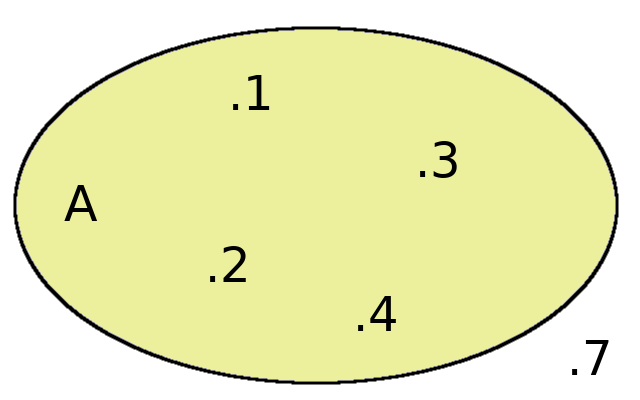
\includegraphics[width=3cm]{diagramadevenn1.png}
   
\end{figure} 

\end{minipage}


               \end{minipage}


     \end{frame}






\end{document}